\documentclass[class=report, crop=false, 12pt,a4paper]{standalone}
\usepackage{enumitem}
\usepackage{multicol}
\usepackage{etoolbox}
\AtBeginEnvironment{quote}{\singlespacing\small}
\usepackage{setspace}
\onehalfspacing
\usepackage{graphicx}
\usepackage{float}
\usepackage{amsmath}
\usepackage{amssymb}
\usepackage{mathtools}
\usepackage{siunitx}
\sisetup{detect-all}
\begin{document}
\section{Control-volume approach}
Recall from thermodynamics that \(\dot{m}_{in} = \dot{m}_{out}\) for a control volume (A c.v. allows heat, work and mass transfer across its boundary). In fluid dynamics different terminology is usually used:
\begin{itemize}[noitemsep]
  \item Closed system = control mass = system (in fluid mechanics).
  \item Open system = control volume.
\end{itemize}
We also know that \(\frac{dm_{cv}}{dt} = \dot{m}_{in} - \dot{m}_{out} \) from thermodynamics. For a \emph{system}, \( \left( \frac{dm}{dt} \right)_{sys} = 0\) since a system is a control mass. 
\section{Simple Reynolds transport theorem}
\begin{equation}
  \frac{DB_{sys}}{Dt} = \frac{\partial B_{cv}}{\partial t} + \dot{B}_{out} - \dot{B}_{in}
\end{equation}
Where $\frac{\partial B_{cv}}{\partial t}$ is how the property changes inside and $\dot{B}_{out} - \dot{B}_{in}$ is what is flowing in and out.
\begin{align}
  \dot{B}_{in} &= b_{in} \dot{m}_{in} = b_{in}\rho_{in}v_{in}A_{in} \textrm{ and}\\
  \dot{B}_{out} &= b_{out} \dot{m}_{out} = b_{out}\rho_{out}v_{out}A_{out}\\
  \therefore \frac{DB_{sys}}{Dt} &= \left( \frac{\partial B}{\partial t} \right)_{cv} + (b \rho v A)_{out} - (b \rho v A)_{in}
\end{align}
This makes an assumption: that the flow is linear across the cross-section, whereas in reality this is not the case.
\begin{align}
  \dot{m} &= \rho v A \rightarrow \textrm{unrealistic}\\
  \dot{m} &= \int_A (\rho v) dA \rightarrow \textrm{realistic} \label{realisticSimpleRTT}
\end{align}
Equation \ref{realisticSimpleRTT} is the integral over different sections and encapsulates that the velocity is changing and that the density may also be changing. If the velocity of the fluid is not in the direction of the pope, then you have to only multiply by a component.
\begin{equation}
  \dot{m} = \int_A (\rho v \cos{\theta})dA 
\end{equation}
Instead of mass, lets do it for $\dot{B}_{in}$ and $\dot{B}_{out}$. 
\begin{align}
  \dot{B}_{out} &= \int_A (b \rho v \cos{\theta})dA\\ 
  \textrm{where } \rho v \cos{\theta} dA &= \dot{m}
\end{align}
Let us define a unit normal vector $\underline{\hat{n}}$ on the exit. Thus:
\begin{align}
  \dot{B}_{out} &= \int_A (b \rho \overline{v} \cdot \underline{\hat{n}}) dA\\
  \overline{v} \cdot \underline{\hat{n}} &= |\overline{v}| \cos{\theta} \textrm{ hence}\\
  &= \dot{B}_{out} - \dot{B}_{in}
\end{align}
As the cross product would produce a negative if the angle is more than \ang{90}.
\begin{align}
  \therefore \dot{B}_{out} - \dot{B}_{in} &= \int_A (b \rho \overline{v}\cdot \underline{\hat{n}})dA\\
  \therefore \left( \frac{DB}{Dt} \right)_{sys} &= \left( \frac{\partial B}{\partial t} \right)_{cv} + \int (b \rho \overline{v}\cdot \underline{\hat{n}}) dA
\end{align}
\section{Reynolds transport theorem: RTT}
\begin{figure}
  \centering
  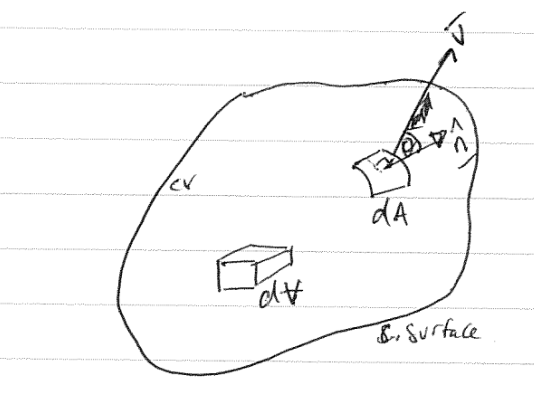
\includegraphics[width = 0.7\textwidth]{../img/RTTDiagram}
  \caption{Diagram to show the Reynolds Transport Theorem.}
\end{figure}
Where:
\begin{itemize}[noitemsep]
  \item $\underline{\hat{n}} =$ unit vector.
  \item $dA =$ area element.
  \item $d\forall =$ volume element.
  \item $B =$ an extensive property.
  \item $b =$ an intensive property.
\end{itemize}
As a reminder the SRTT is:
\begin{equation}
  \left( \frac{DB}{Dt} \right)_{sys} = \left( \frac{\partial B}{\partial t} \right)_{cv} + \dot{B}_{out} - \dot{B}_{in}
\end{equation}
The general form of the RTT is:
\begin{equation}
  \left( \frac{DB}{Dt} \right)_{sys} = \frac{\partial}{\partial t} \int_{cv} (\rho b) d\forall + \int_{cs} (\rho b \overline{v} \cdot \underline{\hat{n}}) dA
\end{equation}
$\rho d \forall =$ mass of $d\forall$ then take an integral to calculate total mass. The change in the property of the C.V. $\int_{cs} (\rho b \overline{v} \cdot \underline{\hat{n}}) dA$ tells us how much B is changing per second. The net flow out of the C.S.

We apply the RTT to 3 cases:
\begin{enumerate}[noitemsep]
  \item Mass conservation.
  \item Newton's second law.
  \item Energy conservation (first law of thermodynamics).
\end{enumerate}
\subsection{RTT and conservation of mass}
The property of consideration is mass: 
\begin{gather}
  B = \textrm{mass} = M
  \therefore b = \frac{B}{\textrm{mass}} = \frac{M}{M} = 1
\end{gather}
Applying these substitutions into RTT
\begin{equation}
  \frac{DM_{sys}}{Dt} = \frac{\partial}{\partial t} \int_{cv} (\rho)d\forall + \int_{cs} (\rho \overline{v} \cdot \underline{\hat{n}}) dA
\end{equation}
By definition, a system = closed system = control mass.
\begin{align}
  \therefore \frac{DM_{sys}}{Dt} &= 0\\
  0 =\frac{\partial M_{cv}}{\partial t} &+ \int_{cs} (\rho v_n) dA\\
  \therefore \frac{\partial M_{cv}}{\partial t} &= - \int_{cs} (\rho v_n) dA
\end{align}
Note: $\int_{cs} (\rho v_n) dA$ is the net mass flow rate through the C.S. out.
\subsection{Example Q}
INSERT
\subsection{RTT and Newton's second law}
\begin{equation}
  \begin{rcases}
    \underline{B} = m \overline{v} = \textrm{linear momentum}&\\
    \underline{b} = \overline{v} = \textrm{velocity}&
  \end{rcases} \textrm{Vectors}
\end{equation}
Substituting this into RTT gives (replacing b with $\overline{v}$).
\begin{equation}
  \frac{D}{Dt}(m\overline{v})_{sys} = \frac{\partial}{\partial t} \int_{cv} (\rho \underline{\overline{v}}) d\forall + \int_{cs} (\rho \overline{v} (\overline{v}\cdot \hat{n})) dA = ?
\end{equation}
Where $\frac{D}{Dt}(m\overline{v})_{sys}$ is the acceleration. M is a constant and hence $m\frac{D}{Dt}\overline{v} = \overline{a} \times m$. Thus, the $? = \sum \overline{F} \leftarrow$ sum of all the forces by Newton's second law. Hence:
\begin{equation}
  \frac{D}{Dt} (m \overline{v})_{sys} = \frac{\partial}{\partial t} \int_{cv} (\rho \overline{\underline{v}}) d\forall + \int_{cs} (\rho \overline{v}(\overline{v} \cdot \hat{n})) dA = \sum \overline{F}
\end{equation}
This is a vector equation and can be split up into x, y and z components. $\frac{\partial}{\partial t} \int_{cv} (\rho \overline{\underline{v}}) d\forall$ is the rate of change of linear momentum inside the C.V. $\int_{cs} (\rho \overline{v}(\overline{v} \cdot \hat{n})) dA$ is the net flow of linear momentum through C.S.
\subsection{Example: mass flow at a pipe junction}
Consider the steady flow in a water pipe joint shown in the diagram.
\begin{figure}[h]
  \centering
  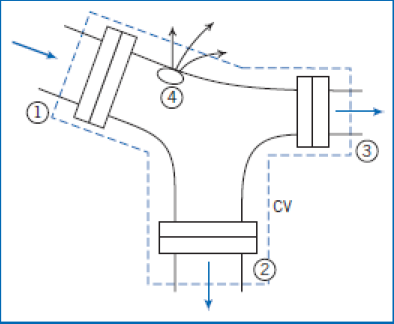
\includegraphics[width = 0.6\textwidth]{../img/waterpipejunction}
  \caption{Water pipe junction.}
\end{figure}
The areas are: $A_1 = 0.2$ \si{\meter\squared}, $A_2 = 0.2$ \si{\meter\squared} and $A_3 = 0.15$ \si{\meter\squared}. In addition, fluid is lost out of a hole at 4, estimated at a rate of 0.1 \si{\meter\cubed\per\second}. The avergae speeds at sections 1 and 3 are $V_1 = 5$ \si{\meter\per\second} and $V_3 = 12$ \si{\meter\per\second} respectively. Find the velocity at section 2.

Given: steady flow of water through the device.
\begin{center}
  \begin{tabular}{|c|c|c|}
    \hline
    $A_1 = 0.2$ \si{\meter\squared} & $A_2 = 0.2$ \si{\meter\squared} &$A_3 = 0.15$ \si{\meter\squared}\\
    \hline
    $V_1 = 5$ \si{\meter\per\second} & $V_3 = 12$ \si{\meter\per\second} & $\rho = 999$ \si{\kg\per\meter\cubed}\\
    \hline
  \end{tabular}
\end{center}
Volume flow rate at 4 $=0.1$ \si{\meter\cubed\per\second}. Find velocity at section 2.

Choose a fixed control volume as shown. Make an assumption that the flow at section 2 is outwards and label the diagram accordingly (if this assumption is incorrect our final result will tell us.) Due to assumptions 2 and 3 below, we may use the following equation:
\begin{equation}
  \sum_{CS} \vec{V} \cdot \vec{A} = 0
\end{equation}
Assumptions:
\begin{itemize}[noitemsep]
  \item Steady flow (given).
  \item Incompressible flow.
  \item Uniform properties at each section.
\end{itemize}
Hence, for the leak:
\begin{equation}
  \vec{V}_1 \cdot \vec{A}_1 + \vec{V}_2 \cdot \vec{A}_2 + \vec{V}_3 \cdot \vec{A}_3 + Q_4 = 0
  \label{exampleRTT1}
\end{equation}
where $Q_4$ is the flow rate out of the leak. Let us examine the first three terms in equation (\ref{exampleRTT1}) and the directions of the velocity vectors.
\begin{figure}
  \centering
  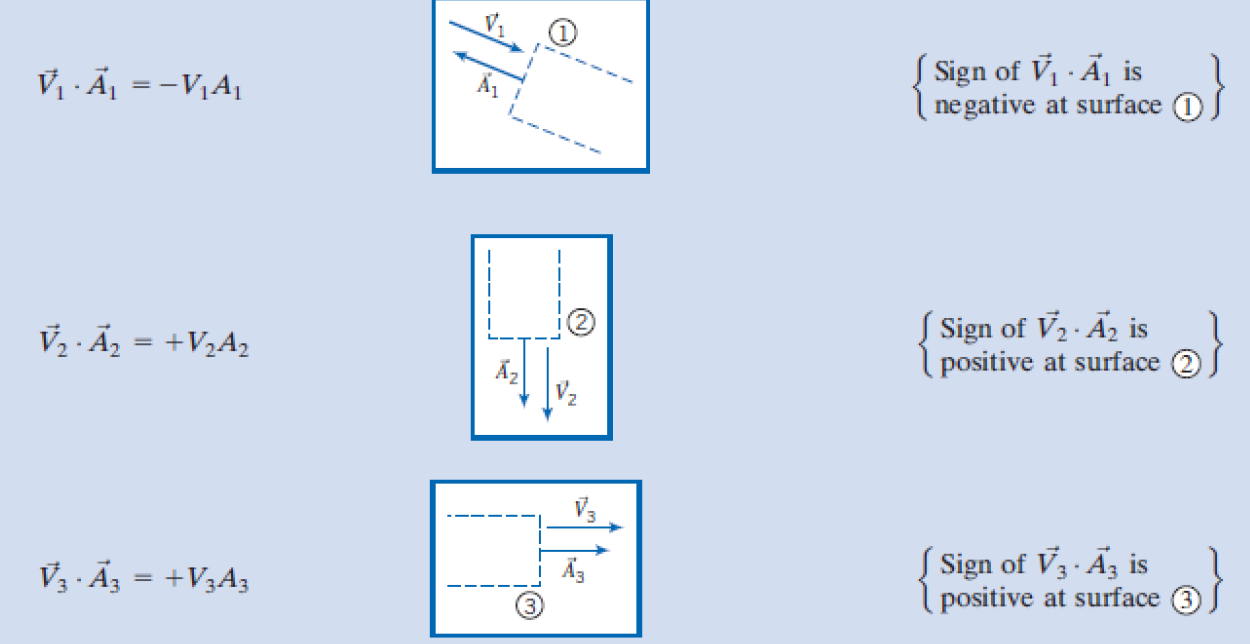
\includegraphics[width = 0.7\textwidth]{../img/RTTexample2}
  \caption{Direction of velocity vectors. }
\end{figure}
Using these results in equation (\ref{exampleRTT1}),
\begin{equation}
  -V_1 A_1 + V_2 A_2 + V_3 A_3 + Q_4 = 0
\end{equation}
or
\begin{align}
  V_2 &= \frac{V_1 A_1 - V_3 A_3 - Q_4}{A_2}\\
  V_2 &= \frac{5\times 0.2 - 12\times 0.15 - 0.1}{0.2}\\
  V_2 &= -4.5 \ \si{\meter\per\second}
\end{align}
Recall that $V_2$ represents the magnitude of the velocity which we assumed was outwards from the control volume. The fact that $V_2$ is negative means that in fact we have an inflow at location 2 - our initial assumption was invalid.

This problem demonstrates use of the sign convention for evaluating $\int_A \vec{V} \cdot d\vec{A}$ or $\sum_{CS} \vec{V} \cdot \vec{A}$. In particular, the area normal is always drawn outwards from the control surface.
\section{Laminar flow and boundary layers}
\subsection{Boundary conditions}
You will generally only come across two types of boundary conditions:
\begin{enumerate}[noitemsep]
  \item No-slip condition: at the point where the fluid touches the boundary, the velocity of the fluid along the boundary is zero. This is the case where the boundary is a solid.
  \item Free surface: there are no viscous forces on the fluid where it touches the boundary, so the speed can take any value. This is the case where there is a liquid-gas boundary and may be called (e.g. for a stream) \emph{open-channel flow.}
\end{enumerate}
\subsection{Laminar flow calculations}
Consider laminar flow between two flat plates. Split the flow into sheets of thickness \(d_{in}\). The top plate moves at constant speed \(v\) and the lower plate is stationary. Here boundary condition (1) applies i.e. fluid at the boundary moves at the speed of the boundary. The top plate has an area \(A\) and the sideways force being applied to it is \(F \therefore \tau = \frac{F}{A} \). If the flow is steady, the forces must balance for each layer. However, the liquid layers must transmit the stress so \(\tau\) is constant throughout the depth. Let us apply our boundary conditions:
\begin{align}
  u_y(0) &= 0 \\ 
  u_y(D) &= v
\end{align}
where D is the vertical distance between the upper and lower plate.
\begin{gather} 
  \therefore \tau = \mu \frac{du_y}{dx} \\
  \left.
    \begin{array}{r}
      \frac{\tau}{\mu} dx = du_y \\
      \frac{\tau}{\mu}\int dx = \int du_y \\
      k + \frac{\tau}{\mu}x = u_y
    \end{array}
  \right\}
  \begin{array}{l}
    u_y = \frac{\tau}{\mu}x + k \\
    0 = \frac{\tau}{\mu}\cdot 0 +k \therefore k = 0 \\
    \textrm{also } \frac{\tau}{\mu} = \frac{v}{D} \rightarrow \tau = \frac{v}{D}\mu
  \end{array}\\
  \therefore u_y = \frac{v}{D}x
\end{gather}
\subsection{Laminar flow between solid boundaries}
In laminar flow, individual particles of fluid follow paths that do not cross those of neighbouring particles. However, there is still a velocity gradient across the flow. Laminar flow is not normally found except in the neighbourhood of a solid boundary, the retarding effect of which causes the transverse velocity gradient. 
\begin{equation} 
  \tau = \mu \left( \frac{\partial u}{\partial y} \right)
\end{equation}
Where \(\tau\) is the resultant shear stress, \(\mu\) is the dynamic viscosity and \(\left( \frac{\partial u}{\partial y} \right)\) is the rate at which the velocity \(u\) increases with the coordinate \(y\) perpendicular to the velocity.

We can use the above to find the required shear stress, if we know the speed the fluid layer thickness and the viscosity:
\begin{equation} 
  \tau = \frac{v}{D}\mu
\end{equation}
\subsubsection{Flow between flat plates example}
Consider two flat plates stuck together with a layer of honey of uniform thickness. Assume laminar flow between the plates. How hard must you pull sideways to separate them at a speed of 1 \si{\cm\per\second}?
\begin{itemize}[noitemsep]
  \item Viscosity of honey = 100 \si{\pascal \second}
  \item Thickness \(D\) = 0.003 \si{\meter}
  \item Speed \(v\) = 0.01 \si{\meter\per\second}
  \item Width = 0.02 \si{\meter}
  \item Area (\(A\)) = width \(\times\) length (\(l\))
\end{itemize}
Assuming that there end effects can be neglected, the stress is equal to the force applied divided by the area. Thus, we can see that the required force decreases as the plates separate.
\begin{align}
  \tau &= \frac{F}{A}\\
  &= \frac{v}{D}x\\
  F &= \frac{v}{D}\mu \cdot A\\
  F &= \frac{0.01}{0.003}100 \cdot 0.02 \cdot l\\
  F &=6.6l
\end{align}
\subsection{Finding shear stress}
The velocity field in a sample of seawater is given below, where A and B are constants:
\begin{equation} 
  u_y = A(B^2-x^2)
\end{equation}
Tiny sea creatures called dinoflagellates emit light when the shear stress in the water around passes a critical level. This is a major cause of bioluminescence at the surface of the ocean. For one particular species, the critical stress level is \(\tau_c = 1 \si{\newton\per\meter\squared}\). The water viscosity is \( \mu = 1.2 \times 10^{-3} \si{\pascal\second} \) and the constants are \(A = -200, \ B=0.1 \). At what x-position in this water sample will the dinoflagellates start to glow?

Remembering: \( \tau = \mu \frac{du_y}{dx} \), we can solve for the case \(\tau_c\).
\begin{align}
  u_y &= -200(0.01-x^2)\\
  u_y &= -2 +200x^2\\
  \frac{du_y}{dx} &= 400x\\
  1 &= 1.2 \cdot 10^{-3} \cdot 400x\\
  x &= 2.08\si{\meter}
\end{align}
\subsection{Laminar flow in pipes}
What is the velocity at different radii in the pipe? We have circular symmetry and a no-slip boundary condition. Flow is being driven by a pressure difference between two ends of the tube. Note that the velocity and the pressure gradient vector point in opposite directions because fluid flows from high to low pressure. We will assume that the flow is fully developed i.e. that the velocity profile is constant along the pipe axis. Consider one cylinder of fluid with an edge at constant radius r. the total pipe radius is R. There is a pressure difference between the two ends of the tube. The total pressure difference is \(\Delta P\) over a length L of tube. The total resultant force parallel to the tube axis must be \(F\cdot A\).
\begin{align}
  Force &= \Delta P \pi r^2\\
  Force &= \frac{dP}{dx}L\pi r^2
\end{align}
The force provided by the pressure difference must be equal to the shear stress on the outside of the cylinder, since the forces are balanced.
\begin{equation} 
  Force = 2\tau \pi r L 
\end{equation}
Equating these two forces:
\begin{align}
  \frac{dP}{dx}L\pi r^2 &= 2\tau \pi r L\\
  \tau &= \frac{r}{2} \frac{dP}{dx}
\end{align}
We can relate the shear stress at the cylinder surface to the velocity change with radius there:
\begin{align}
  \tau &= \mu \frac{du}{dr}\\
  \tau &= \mu \frac{du}{dr}\\
  &= \frac{r}{2} \frac{dP}{dx}\\
  \frac{du}{dr} &= \frac{r}{2\mu} \frac{dP}{dx}
\end{align}
Now we can integrate to \(u\):
\begin{align}
  u &= \int \left( \frac{r}{2\mu} \frac{dP}{dr} \right) dr\\
  u &= \frac{1}{2\mu} \frac{dP}{dx} \int (r) dr\\
  u &= \frac{1}{2\mu} \frac{dP}{dx} \frac{1}{2}r^2 +k
\end{align}
Applying the no-slip boundary condition, \( u(R) = 0\):
\begin{align}
  0 &= \frac{1}{2\mu} \frac{dP}{dx} \frac{1}{2} R^2 + k\\
  k &= \frac{-1}{4\mu} \frac{dP}{dx} R^2 \\
  \therefore u &= \frac{-1}{4\mu}\frac{dP}{dx}(R^2 - r^2)
\end{align}
How can we use this? The maximum speed is at the centre of the pipe, where r = 0. We know the flow speed with radius, so we can integrate this to find the total volume flow.
\begin{align}
  u_{max} &= \frac{-1}{4\mu}\frac{dP}{dx} R^2\\
  Q &= \int^R_0 \left( u(r)\cdot 2\pi r \right) dr\\
  Q &= \int^R_0 \left( \frac{-1}{4\mu} \frac{dP}{dt}(R^2 - r^2) \cdot 2\pi r \right) dr 
\end{align}
The average flow speed is the total volume flow rate divided by the cross sectional area:
\begin{equation} 
  u_{mean} = \frac{Q}{\pi r^2}
\end{equation}
\begin{center}
  Laminar flow through pipes of circular cross section is often called Hagan-Poiseulle flow.
\end{center}
\end{document}